\documentclass[12pt]{article}
\usepackage[utf8]{inputenc}
\usepackage[english,russian]{babel}
\usepackage[12pt]{extsizes}
\usepackage{booktabs}
\usepackage{graphicx}
\usepackage{graphicx,psfrag}
\usepackage{cite}
\usepackage{sectsty}
\usepackage{amsmath, esint, setspace, fancyhdr, amsfonts, bookmark, blindtext}

\graphicspath{{Figures/}}
\DeclareGraphicsExtensions{.pdf,.png,.jpg}
\setlength{\textheight}{8in}
\setlength{\textwidth}{6.6in}
\setlength{\headheight}{0in}
\setlength{\headsep}{0.2in}
\setlength{\topmargin}{0in}
\setlength{\oddsidemargin}{0in}
\setlength{\evensidemargin}{0in}
\setlength{\parindent}{.3in}
\renewcommand{\baselinestretch}{1.4}

\doublespacing
\newcommand{\threeimage}[6]{
\begin{figure}[h!]  
    \centering 
    \subfigure[]{
        \includegraphics[width=0.25\linewidth, height=0.25\linewidth]{#1} 
        \label{fig_f_ #1} }  
        %\hspace{4ex}
    \subfigure[]{
    \includegraphics[width=0.25\linewidth, height=0.25\linewidth]{#2} 
    \label{fig_f_ #2} }
   % \hspace{4ex}
    \subfigure[]{ 
        \includegraphics[width=0.25\linewidth, height=0.25\linewidth]{#3} 
        \label{fig_f_ #3} }  
    \caption{ 
    \subref{fig_f_ #1} #4; 
    \subref{fig_f_ #2} #5; 
    \subref{fig_f_ #3} #6} 
    \label{fig:f_ #1#2#3}
\end{figure}}


\begin{document}

\definecolor{comment}{rgb}{0.71, 0.29, 0.29}

\begin{titlepage}

\begin{center}
Санкт-Петербургский политехнический университет Петра Великого\\
Институт прикладной математики и механики\\
Кафедра прикладной математики\\
\hrulefill
\end{center}

\begin{flushleft}
\rule{9cm}{0pt} {Работа допущена к защите}\\
\rule{9cm}{0pt} Зав. кафедрой\\
\rule{9cm}{0pt} \rule{2.5cm}{0.5pt} {\bfseries{М. Е. Фролов }}\\
\rule{9cm}{0pt} "\rule{.9cm}{0.5pt}" \rule{4cm}{0.5pt}
\end{flushleft}

\vspace{1.5cm}

\begin{center}
{\large {\bfseries ОТЧЕТ\\
о научно-исследовательской работе}}\\

\bigskip \bfseries{Тема:} {\bfseries \emph{Классификация саженцев растений}}
\end{center}

\vspace{1.cm}

\begin{flushleft}
Направление: 01.03.02 Прикладная математика и информатика

\vspace{1.cm}

Выполнил студент гр. 33631/4 \hfill{Камалетдинова Ю.А.} \\ 

\vspace{0.2cm} Руководитель \hfill{Яковлев Д.В.}

\end{flushleft}

\vspace{1.5cm}

\begin{center}
Санкт-Петербург\\
2019
\end{center}

\end{titlepage}


\tableofcontents
\addtocontents{toc}{~\hfill\par}
\vfill ~
\setcounter{section}{0}
\newpage 

\section{Введение}

\indent{\indent Потребность в сельскохозяйственных продуктах увеличивается с каждым днем, как и растет население планеты Земля. Часть работ выполняют люди, и силы уходят на контроль качества выращиваемых культур. Мы сможем использовать временные и природные ресурсы более бережно и экономно, увеличим урожаи, если научимся дифференцировать благородные культуры и отличать их от сорняков без помощи человека. }

\indent{ В такой ситуации естественным образом приходит мысль об автоматизации процессов, например, классификация саженцев по фотоснимкам. Возникает мысль задействовать нейросети, что обосновано преимуществами, но также они обладают недостатками в виде вычислительных затрат. }

\indent{  Возможно использовать алгоритмы другой группы, но они требуют более тонкой настройки для достижения сопоставимого результата, а иногда вовсе не могут быть улучшены. В данной работе поставим задачу классификации растений и решим ее методом опорных векторов. }

\section{Анализ набора данных}
\subsection{Первичный взгляд на данные}

\indent{\indentИсследуемый набор данных был собран группой Орхусского университета по обработке сигналов в сотрудничестве в Университетом Южной Дании. Этапы создания коллекции описаны с статье \cite{bib_1}. Набор содержит приблизительно 960 уникальных изображений растений 12 видов, находящихся на разных стадиях роста. }\\
\indent{Изучимы исходные данные. Построим образцы каждого класса в виде сетки}

\begin{figure}[h]
	\centering
	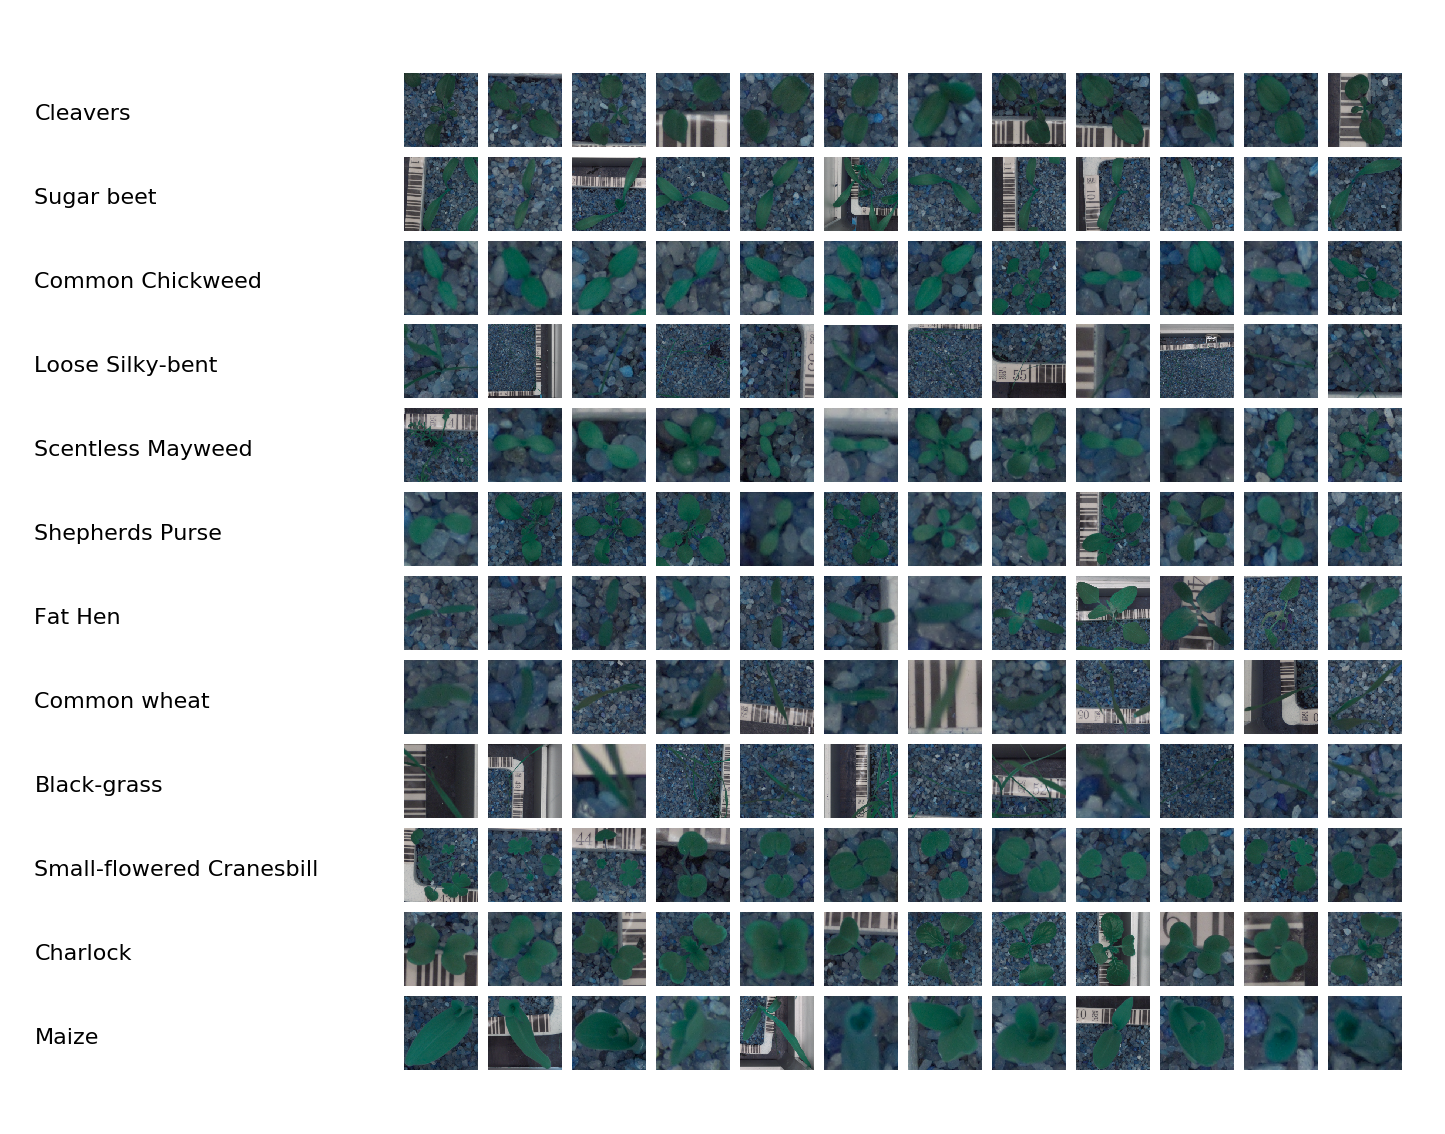
\includegraphics[width=16.cm, height=12.cm]{first_view_grid_1}
	\caption{Образцы растений каждого вида (построчно)}
	\label{fig_1}
\end{figure}

\indent{ Проанализировав снимки, можно сделать некоторые выводы:}
\begin{itemize}
	\item {Исходные изображения уже кадрированы и не требуют дополнительной обрезки 
	\begin{figure}[h!]
		\centering
		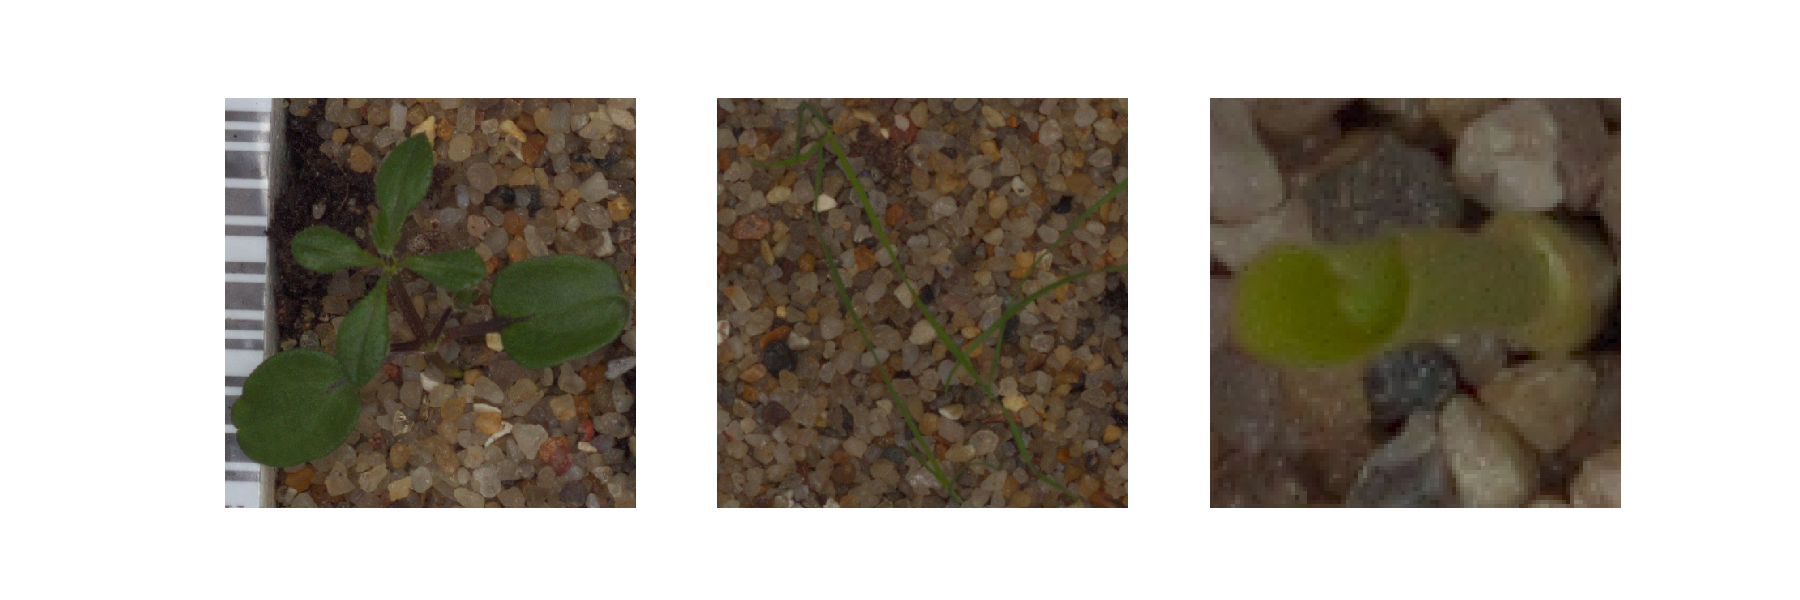
\includegraphics[width=13.cm, height=4.cm]{first_view_three_1}
		\caption{Примеры исходных изображений}
		\label{fig_2}
	\end{figure}
	}
	\item Разрешения изображений варьируются от 50х50px до 2000х2000px, поэтому необходимо привести весь набор к единому разрешению, иначе для каждого изображения значения его признаков будут находиться в разных пределах, что не позволит решить задачу классификации
	\item Данные не сбалансированы: от 221 до 654 размеченных образцов каждого класса
	\item Фон на снимках различен, необходимо выбрать спосбоб сегментации, наиболее подходящий для большинства
\end{itemize}

\subsection{Загрузка изображений}

\subsubsection{Представление данных}

\indent{\indent Библиотека OpenCV использует цветовую модель BGR (Blue Green Red) для представления цветных изображений. Каждый пиксель характеризуется составляющими синей, зеленой и красной компонентами.}

\subsubsection{Изменение разрешения}

\indent{\indent Загрузив изображение, изменим его разрешение до 200х200px. Воспользуемся алгоритмом билинейной интерполяции: в случае уменьшения размера новый пиксель изображения представляет собой взвешенную сумму соседних пикселей исходного и наоборот в случае увеличения разрешения.} 

\subsection{Сегментация}

\indent{\indent Заметим, что все представленные растения окрашены в зеленый цвет. Поэтому мы можем создать маску, фильтрующую диапазон зеленых оттенков и удаляющую пиксели остальных цветов. Для реализации воспользуемся библиотекой компьютерного зрения OpenCV \cite{bib_2} и библиотекой для вычислений Numpy \cite{bib_3} языка программирования Python.}

\indent{ Воспользуемся цветовой моделью HSV (Hue Saturation Value) \ref{fig_3}. В формате BGR значение каждой компоненты зависит от количества света, попадающего на объект. HSV же позволяет разграничить информацию о цвете и яркости. Оттенок, насыщенность и интенсивность позволяют задать нижнюю и верхнюю границы оттенков некоторого цвета, в данном случае –– зеленого.}

\begin{figure}[h]
	\centering
	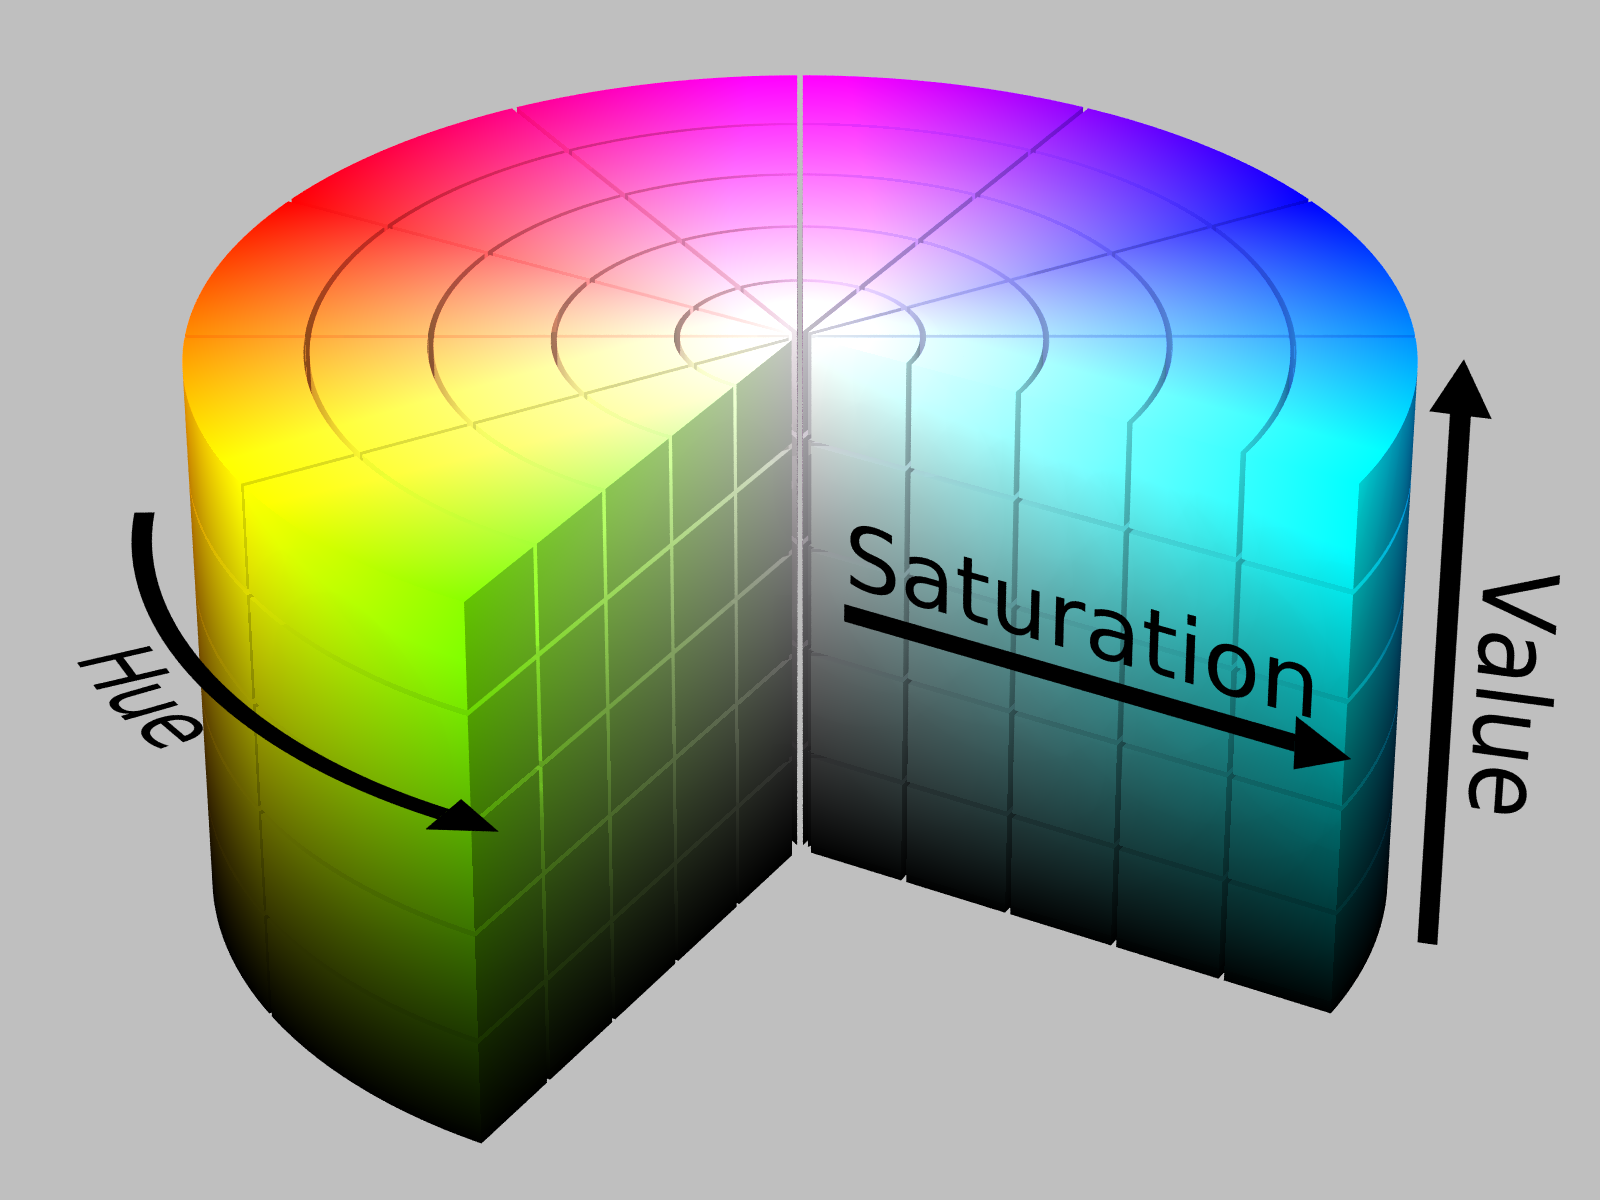
\includegraphics[width=7cm, height=5cm]{hsv}
	\caption{Цветовая модель HSV}
	\label{fig_3}
\end{figure}

\indent{Пометим пиксели, находящиеся в зеленом диапазоне и получим цветовую маску. Теперь применим операцию логического умножения к исходному изображению, присвоим значениям пикселей фона значение черного цвета и получим сегментированное растение}

\threeimage{seg_step_1}{seg_step_2}{seg_step_3}{Исходное изображение}{Маска}{Сегментированное изображение}

\subsection{Удаление шума}

\indent{\indent Сегментация не всегда происходит хорошо, как на примере \ref{fig_f_ seg_step_3}. Небольшие участки фона могут попадать в диапазон зеленых значений, что вызывает искажение бинарной маски, и получается эффект, представленный на рисунке ниже}

\begin{figure}[h]
	\centering
	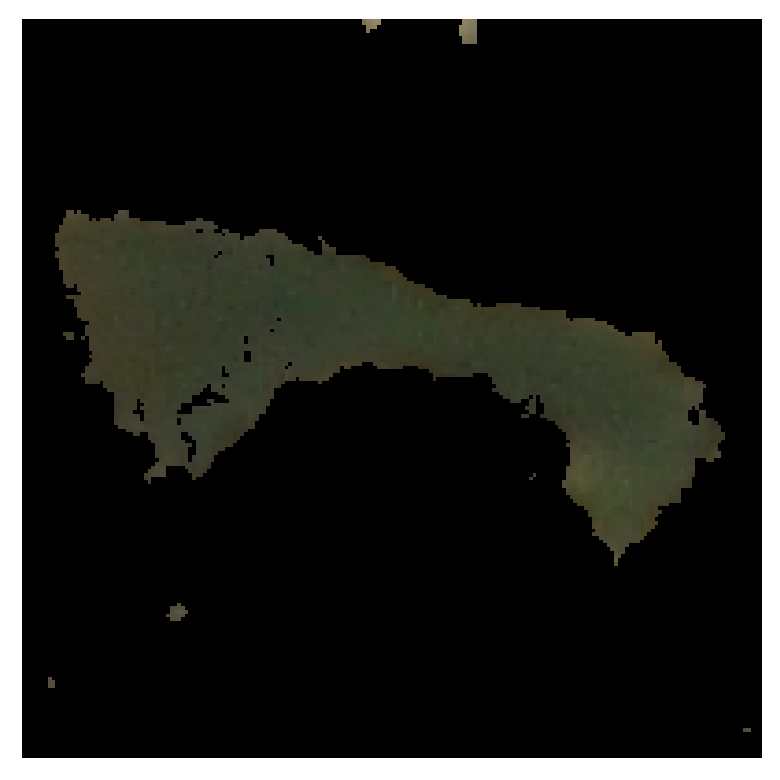
\includegraphics[width=7.cm, height=7.cm]{seg_no_morph_1}
	\caption{Искажения при сегментации}
	\label{fig_4}
\end{figure}

\indent{Такие недостатки можно устранить при помощи морфологических операций –– нелинейных преобразованиях,  связанных с формой и структурой некоторого объекта, в данном случае, изображения. При обработке изображений морфология используется для исследования взаимодействия изображения с определенным структурирующим элементом –– ядром –– с помощью морфологических операций. Ядро итерируется по всему изображению и сравнивается с окрестностью пикселей, что описано в источнике \cite{bib_4}. }

\indent{ Для улучшения сегментации применим операцию морфологического закрытия –– комбинацию операций дилатации и эрозии.}

\indent{ Эрозия бинарного изображения $f$ ядром $s$ (обозначается $f \ominus s$) производит новое бинарное изображение $g = f \ominus s$ с единицами на всех позициях $(x, y)$ ядра, где оно полностью совпадает с исходным изображением $f$, то есть $g(x, y) = 1$, если $s$ поэлементно совпадает с участком $f$ и $0$ в другом случае, для всех координат пикселей $(x, y)$}

\begin{figure}[h]
	\centering
	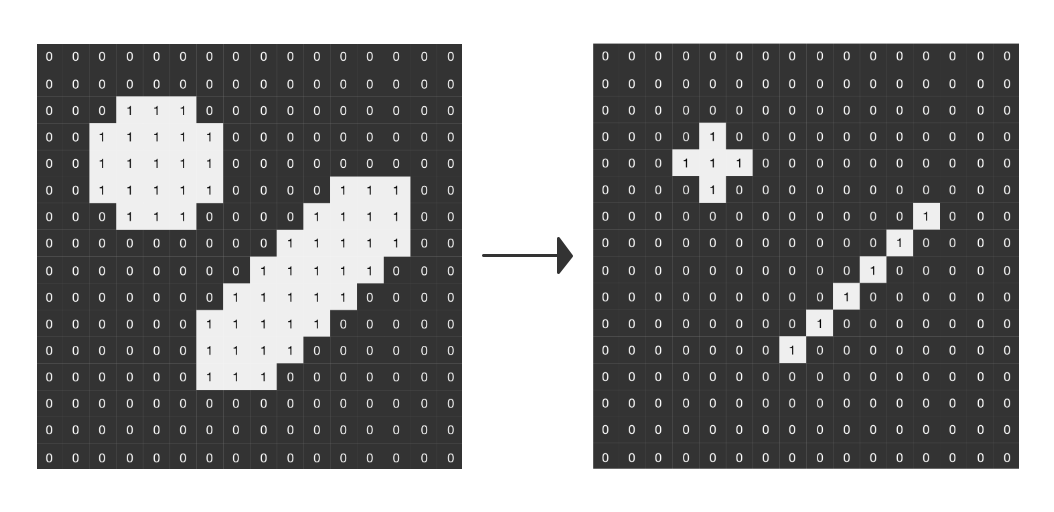
\includegraphics[width=10.cm, height=5.cm]{erosion}
	\caption{Эрозия с квадратным ядром 3х3}
	\label{fig_5}
\end{figure}

\indent{ Дилатация бинарного изображения $f$ ядром $s$ (обозначается $f \oplus s$) производит новое бинарное изображение $g = f \oplus s$ с единицами на всех позициях $(x, y)$ ядра, где оно совпадает с исходным изображением $f$ хотя бы в одной позиции, то есть $g(x, y) = 1$, если $s$ совпадает хотя бы в одной позиции с участком $f$ и $0$ в другом случае, для всех координат пикселей $(x, y)$}

\begin{figure}[h!]
	\centering
	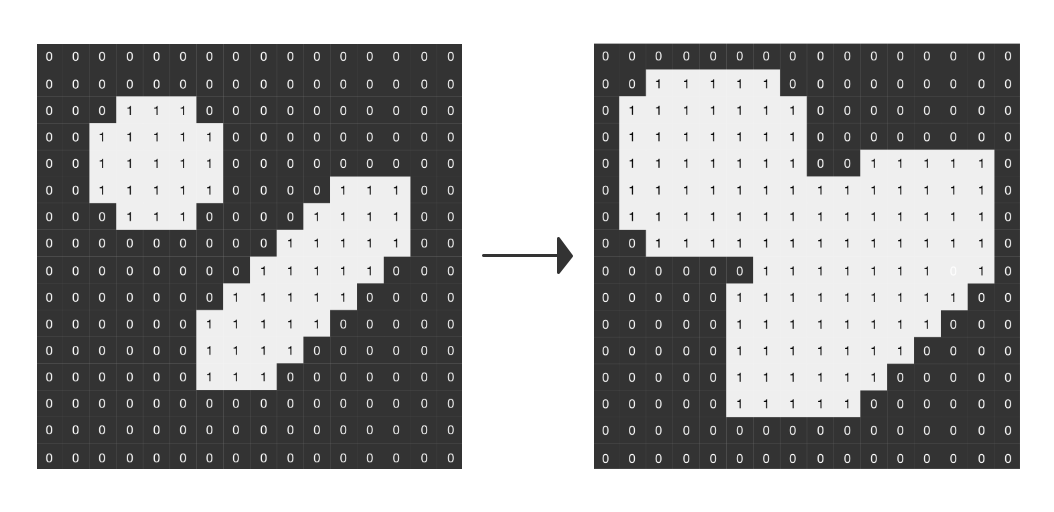
\includegraphics[width=10.cm, height=5.cm]{dilation}
	\caption{Дилатация с квадратным ядром 3х3}
	\label{fig_6}
\end{figure}

%\vspace{1.cm}
\indent{ Теперь можем определить операцию закрытия изображения $f$ ядром $s$ как $f \bullet s = (f \oplus s) \ominus s$. Струкрутрный элемент может быть любой формы, и его выбор зависит от формы недостатков, которые требуется устранить.}

\indent{ Применим операцию закрытия к изображению \ref{fig_4}, выбрав эллиптическое ядро размером 6x6px и удалим оставшиеся объекты площадью менее 160px}

\begin{figure}[h]
	\centering
	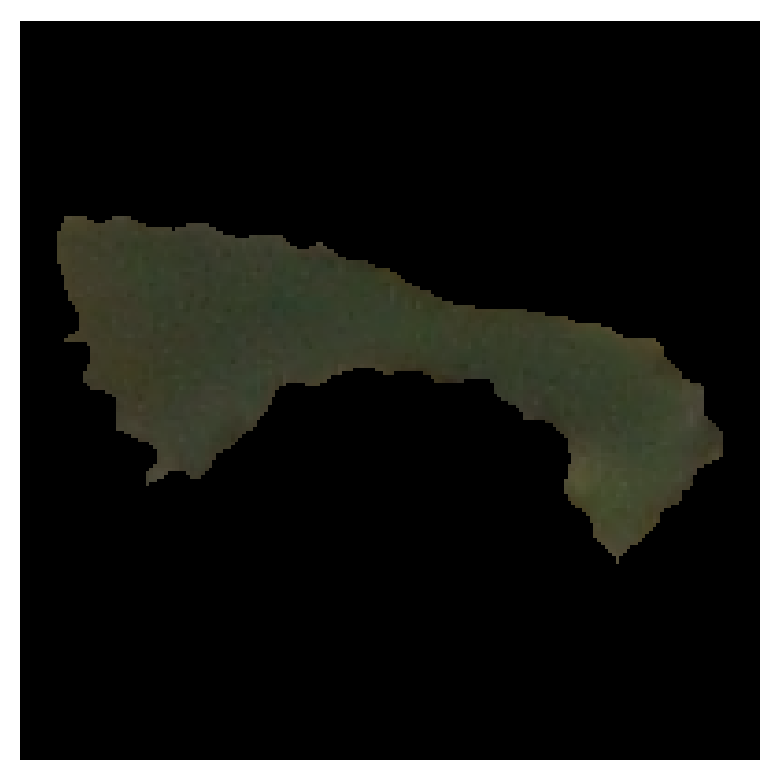
\includegraphics[width=6.cm, height=6.cm]{seg_morph_1}
	\caption{Изображение после закрытия маски}
	\label{fig_7}
\end{figure}

\indent{ Растение на изображении \ref{fig_7} не имеет полостей, а фон очищен от не относящихся к растению элементов. Но морфологическое закрытие не всегда однозначно хорошо действует на изображения. Рассмотрим результат работы над изображением класса Метлица обыкновенная (\textit{англ. Loose silky-bent}): }

\begin{figure}[h]
	\centering
    \subfigure[До морфологического закрытия]{
		{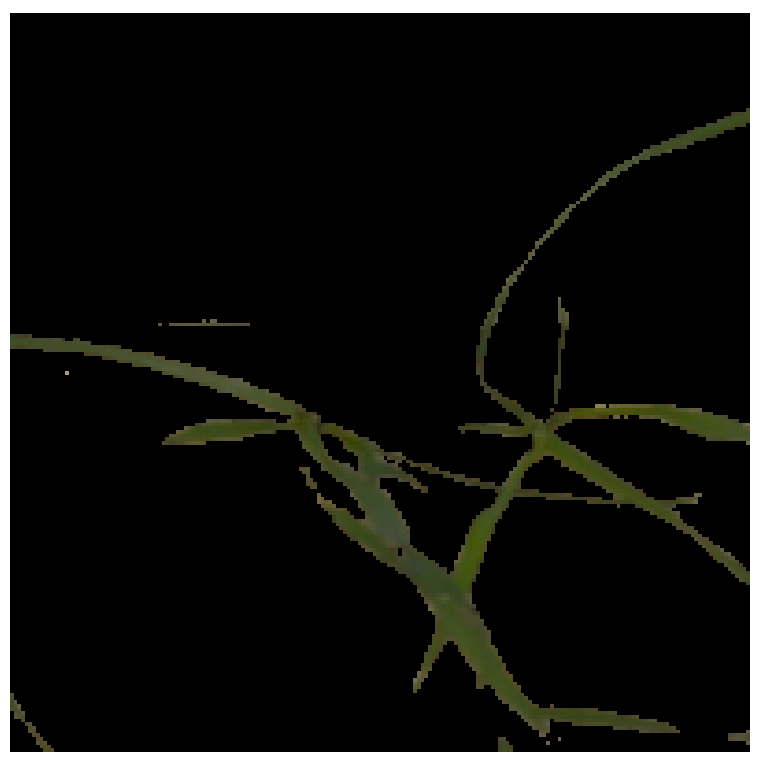
\includegraphics[width=6cm, height=6cm]{seg_no_closure_good_1} 
		\label{fig_7_1_a}}
	}
    \qquad
    \subfigure[После морфологического закрытия]{
		{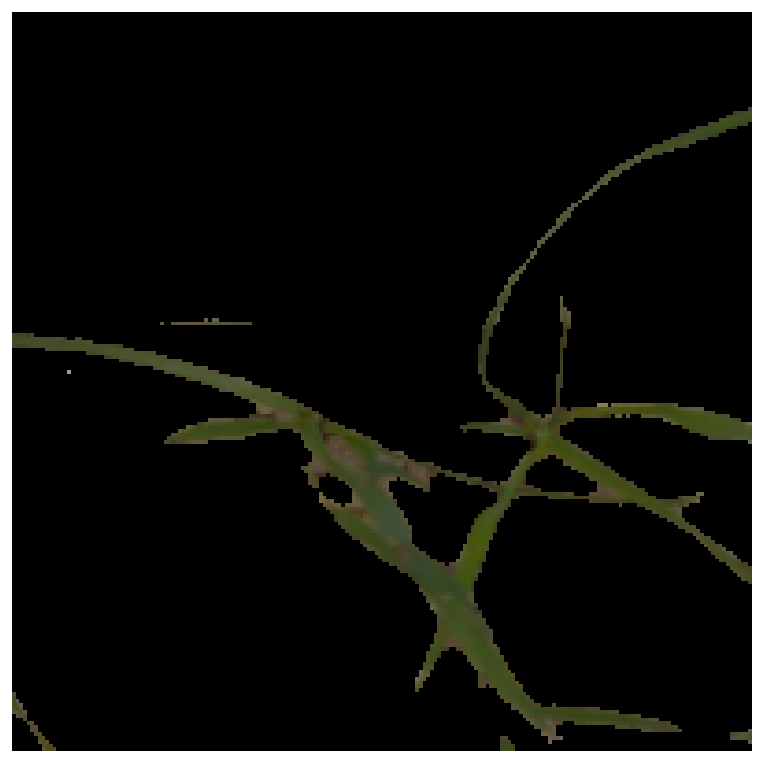
\includegraphics[width=6cm, height=6cm]{seg_with_closure_bad_1} 
		\label{fig_7_1_b}}
	}
    \caption{Пример с ухудшением сегментации}%
    \label{fig_7_1}
\end{figure}

\indent{ На \ref{fig_7_1_b} заметно, что полости, соответвтующие фону, были восстановлены, что не соответствует желаемому результату. Поскольку характеристики ядра и количество итераций определяются однажды и их нельзя изменять адаптивно, то мы не будем применять операцию морфологического закрытия. Ограничимся удалением объектов, чьи контуры ограничивают малую площадь. }


\section{Извлечение признаков}

\indent{\indent Признак в задаче классификации изображений –– это информация, позволяющая решить, к какому заданному классу относится объект. Предположим, что каждый пиксель фотографии –– это его признак. Тогда каждая фотография разрешением 200х200px будет иметь 40000 признаков, к тому же, исходный набор данных –– это более 4000 образцов. Решение задачи не только требует больших вычислительных затрат, но и влечет неспособность алгоритма к обобщению –– переобучение. Более того, часть пикселей вообще не характеризует признаки растения.}

\indent{ Для решения этой проблемы необходимо выбрать признаки с такими свойствами:}
\begin{itemize}
	\item Небольшая размерность пространства признаков
	\item Признаки не должны сильно коррелировать между собой
	\item Набор признаков позволяет классифицировать объект
\end{itemize}

\subsection{Цветовые признаки}

\indent{\indent Чтобы установить сходство, рассчитаем цветовые моменты, характеризующие распределение цвета на изображении. Пусть $\{x^{(k)}\}_{i=1}^N$, где $k = 1 (= R), 2 (= G), 3 (= B)$ –– номер канала цветового пространства RGB, $N$ –– число пикселей изображения, $x^{(k)_i}$ –– $i$-ый пиксель $k$-го канала. Определим характеристики}

\begin{equation}
	\label{eq_1}
	\overline{x^{(k)}} = \frac{1}{N}\sum_{i=1}^{N}x^{(k)}_i \text{ –– выборочное среднее}
\end{equation}

\begin{equation}
	\label{eq_2}
	 s^{(k)} = \sqrt{\frac{1}{N}\sum_{i=1}^{N}(x^{(k)}_i - \overline{x^{(k)}})^2} \text{ –– выборочное стандартное отклонение}
\end{equation}

\indent{Разделим изображение поканально, как на рисунке \ref{fig_8}, и рассчитаем \eqref{eq_1}, \eqref{eq_2}}

\vspace{2.cm}

\begin{figure}[h!]
	\centering
	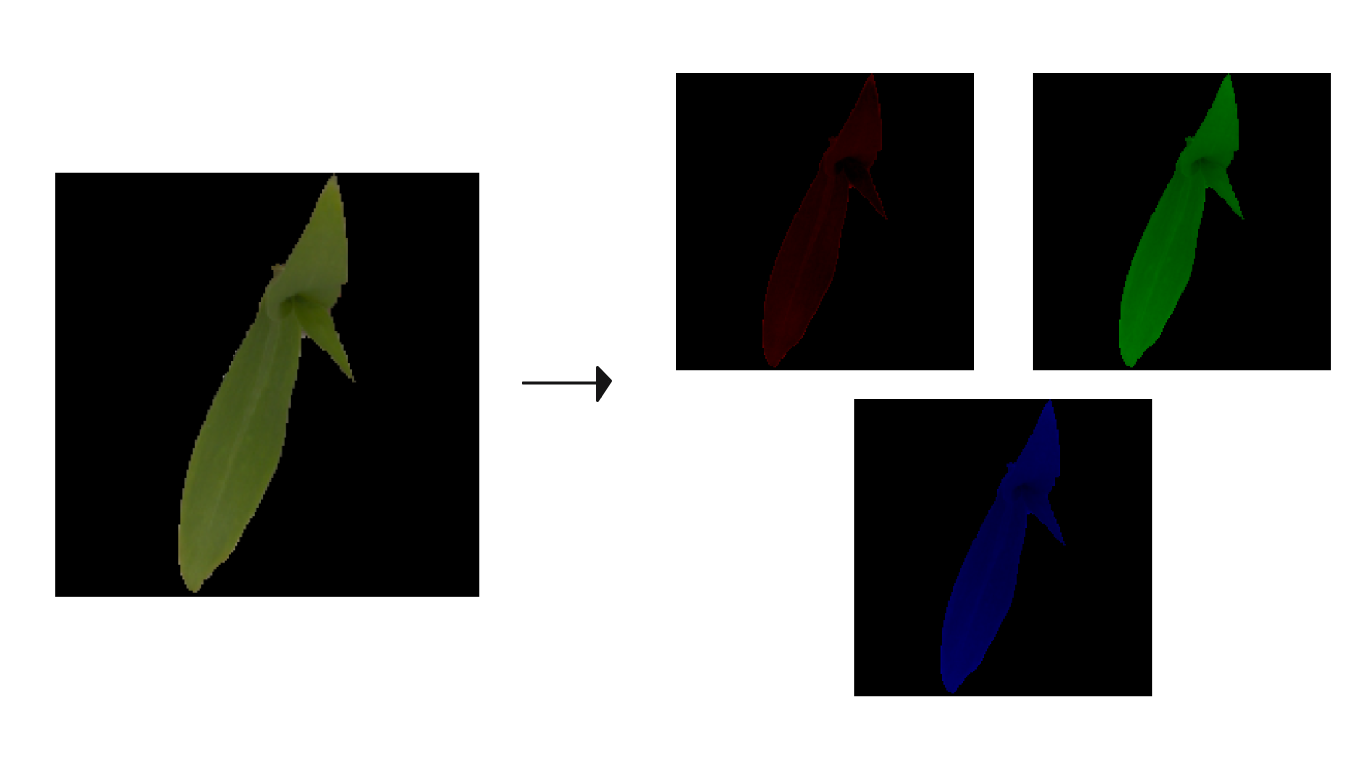
\includegraphics[width=15.cm, height=8.cm]{to_rgb_sample_1}
	\caption{Разложение по каналам R, G, B}
	\label{fig_8}
\end{figure}

\subsection{Признаки формы}

\indent{\indent Не только цвет является важным признаком при классификации. Больше информации можно узнать, выделив признаки формы.}

\subsubsection{Количество ограничивающих контуров}

\indent{\indent В результате сегментации некоторые классы образцов разделяются на несколько объектов. Количество таких объектов –– один из приклаков класса. Для извлечения контуров воспользуемся алгоритмом трассировки границ, описанном в статье \cite{bib_6} и реализованном в открытой библиотеке OpenCV \cite{bib_2} для языка программирования Python. Конуры и все использующие их далее характеристики не учитываются, если ограничиваемая площадь менее 150px$^2$ (установлено эмпирически для изображения 200х200px).}

\subsubsection{Общая площадь}

\indent{\indent Величина составляет сумму всех площадей, ограниченных контурами. Площади вычисляются по формуле Грина по замкнутому контуру, алгоритм реализован в библиотеке OpenCV \cite{bib_2}.}

\subsubsection{Максимальная площадь}

\indent{\indent Представляет собой максимальный по маскимальную площадь, ограничиваюмую контуром.}

\subsubsection{Периметр}

\indent{\indent Вычисляется для контура максимальной длины среди найденных.}

\subsubsection{Мера прямоугольности}

\indent{\indent Для вычисления меры прямоугольности требуется построить наименьший ограничивающий прямоугольник –– множество точек двумерного пространства с наименьшей площадью, включающего в себя все точки объекта-рстения. Тогда рассчитаем характеристику:}
\begin{equation}
	A = \frac{d_{min}}{d_{max}} \text{ –– мера прямоугольности}
	\label{eq_3}
\end{equation}
, где $d_{min}$ и $d_{max}$ –– меньшая и большая стороны прямоугольника соответственно.

\subsubsection{Мера округлости}

\indent{\indent Характеристика показывает, насколько большую площадь ограничивает периметр объекта. Мера округлости круга достигает максимального значения и равна единице.}

\begin{equation}
	f_{circ} = \frac{4 \pi A}{P^2} \text{ –– мера округлости,} 
	\label{eq_4}
\end{equation}
где $P$ –– периметр контура, ограничивающего объект, $A$ –– площадь объекта

\indent{Построим корреляционную матрицу описанных признаков и изобразим ее в виде тепловой карты:}

\begin{figure}[h!]
	\centering
	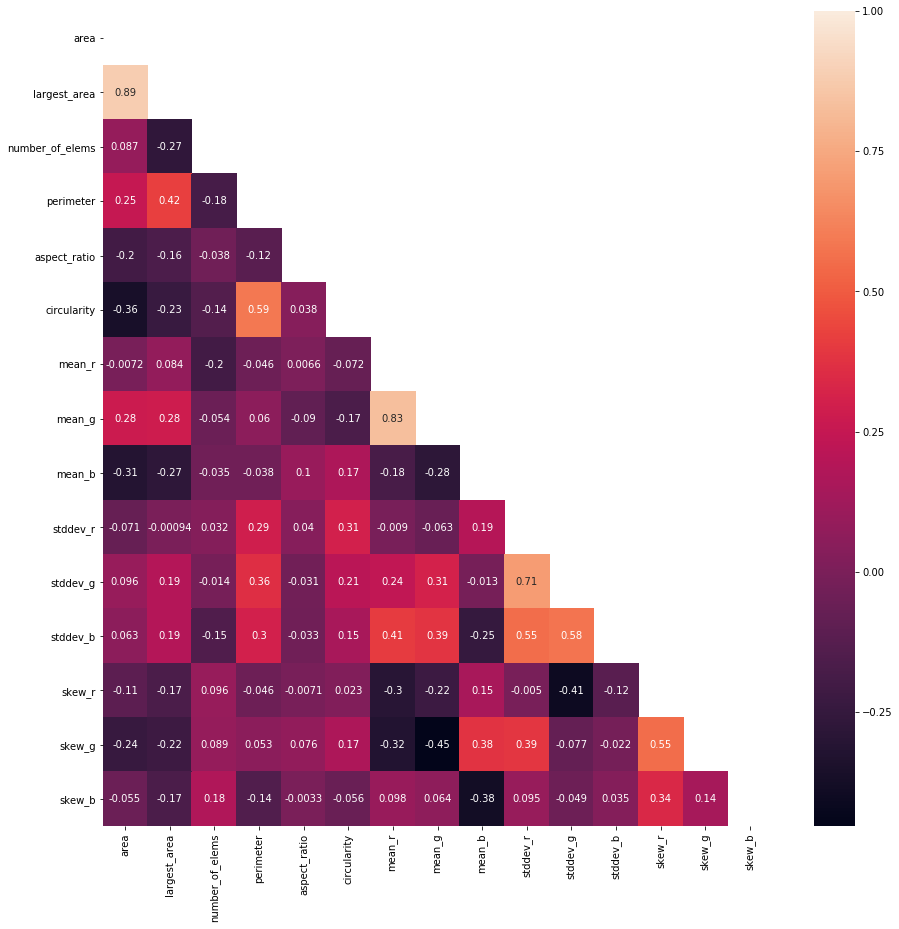
\includegraphics[width=15.cm, height=13.5cm]{corr_heatmap_1}
	\caption{Матрица корреляций признаков}
	\label{fig_corr_matrix}
\end{figure}

\indent{ На основе данных на рисунке \ref{fig_corr_matrix} заключаем, что наиболее линейно зависимы признаки общей площади (area) и максимальная площадь (largest area), но это справедливо не для всех классов в виду преобладания растений, ограниченных одним контуром, поэтому из рассмотрения признак максимальной площади не исключается.}

\section{Классификация}

\subsection{Метод опорных векторов}

\indent{\indent Метод опорных векторов (\textit{англ. Support vector machine, SVM}) –– алгоритм бинарной классификации, основанный на построении разделяющей гиперплоскости с зазором. Алгоритм метода описан в библиотеке Scikit-learn \cite{bib_7} для языка программирования Python.}

\indent{ Пусть $\{(x_i, y_i)\}_{i=1}^l$ –– обучающая выборка, где $x_i \in \mathbb{R}^n$ –– признак объекта, $y \in \{-1, 1\}^l$ –– вектор меток принадлежности классу.  Так как в общем случае гарантировать линейную разделимость выборки невозможно, сформулируем задачу минимизации с дополнительным параметром (\textit{мягким зазором}):}

\begin{equation}
	\min_{w, b, \xi} \;\; \frac{1}{2}w^T w + C\sum_{i=1}^{l} \xi_i 
	\label{eq_5}
\end{equation}
при условиях 
\begin{equation}
	y_i(w^T \phi(x_i) + b) \ge 1 - \xi_i, \\
	\xi_i \ge 0,
	\label{eq_6}
\end{equation}
где $\phi(x_i)$ –– отображение пространства признаков в пространство большей размерности, $\xi_i$ –– поправка, ослабляющая границы классов. Коэффициент $C > 0$ определяет, насколько велик зазор разделяющей гиперплоскости.

\indent{ Определим непрерывную функцию ядра как  $K(x_i, x_j) = \phi(x_i)^T \phi(x_j)$, представляющую собой пары скалярных произведений. В данной работе выберем гауссово ядро с радиальной базовой функцией (\textit{англ.} Radial basis function, RBF):}

\begin{equation}
	K(x_i, x_j) = \exp(\gamma ||x_i - x_j||^2),
	\label{eq_7}
\end{equation}
где $\gamma$ –– параметр ядра

\indent{ Ядро RBF обладает преимуществами перед другими ядрами:}
\begin{itemize}
	\item Позволяет решить задачу \eqref{eq_5} с условиями \eqref{eq_6} в случае, когда выборка не разделима линейно
	\item Один параметр –– $\gamma$, контролирует степень влияния признаков на границу решения
	\item Значения ядра $K(x_i, x_j)$ лежат в пределах $(0, 1]$, не обращаются в 0 и не уходят в бесконечность
\end{itemize}

\indent{ Определим гиперпараметры –– это параметры, которые определяются однажды и не меняются в ходе обучения классификатора. В данной задаче такими параметрами являются $C$ и $\gamma$. Подбор гиперпараметров осуществен с помощью кросс-валидации и поиска по сетке, описанных в статье \cite{bib_8}.}

\indent{Алгоритм SVM чувствителен к неотмасштабированным данным, особенно в случае использования ядра RBF, представляющего собой Евклидово расстояние \eqref{eq_7}. В случае, когда значения свойств находятся в разных интервалах, незначительное отличие в большем может вывести за пределы значений второго свойства. Переведем все значения в отрезок $[0, 1]$:}

\begin{equation}
	z_{i_j} = \frac{x_{i_j} - \min_{i = 1, \dots, l}(x_{i_j})}{\max_{i = 1, \dots, l}(x_{i_j}) - \min_{i = 1, \dots, l}(x_{i_j})}
	\label{eq_8}
\end{equation}

\section{Результаты исследований}
\subsection{Метрика}

\indent{\indentКачество полученным результатов будем оценивать с помощью микро-усредненной F-меры.}

\indent{F-мера –– это гармоническое среднее между точностью и полнотой:}

\begin{equation}
	F = 2 \; \frac{precision * recall}{precision + recall}
	\label{eq_9}
\end{equation}
\begin{equation}
	precision = \frac{TP}{TP + FP}
	\label{eq_10}
\end{equation}
\begin{equation}
	recall = \frac{TP}{TP + FN},
	\label{eq_11}
\end{equation}
$TP \; (True \;Positives)$ –– истино положительные, \\
$FP \; (False \;Positives)$ –– ложно положительные, \\
$FN \; (False \;Negatives)$ –– ложно отрицательные классифицированные объекты \\

\indent{В случае микро-усреднения характеристики TP, FP, FN усредняются для каждого класса, далее вычисляется F-мера по формуле \eqref{eq_9}. Выбор такой метрики обоснован тем, что классы не сбалансированы по объему данных, и в данном случае влияние классов уменьшается за счет усреднения по характеристикам классификации, а не по F-мерам.}

\indent{Представим общие результаты в виде таблицы:}

\begin{figure}[h!]
	\centering
	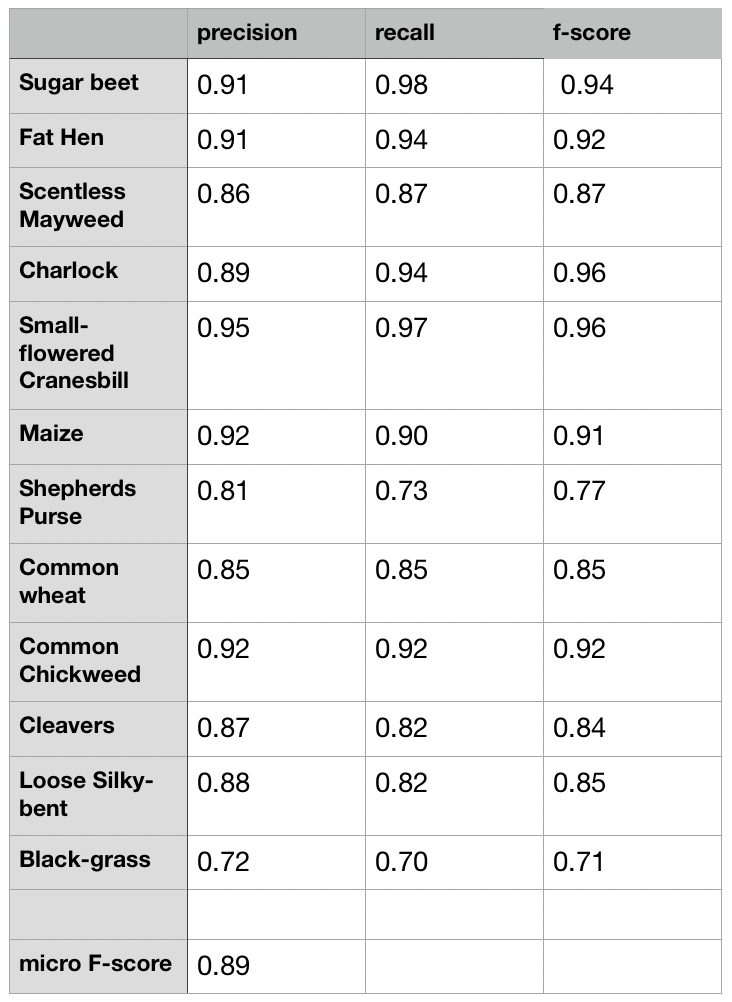
\includegraphics[width=8.cm, height=11.5cm]{metrics_1}
	\caption{Поклассовые характеристики и общая метрика}
	\label{fig_metrics}
\end{figure}

\subsection{Вывод}

\indent{\indentОбратимся к таблице \ref{fig_metrics}. Менее успешно удалось классифицировать объекты класса \textit{Black-grass}. Результат обусловлен тем, что визуально отличить его образец от образца \textit{Loose Silky-bent} довольно затруднительно:}

\begin{figure}[h]
	\centering
    \subfigure[\textit{Black grass}]{
		{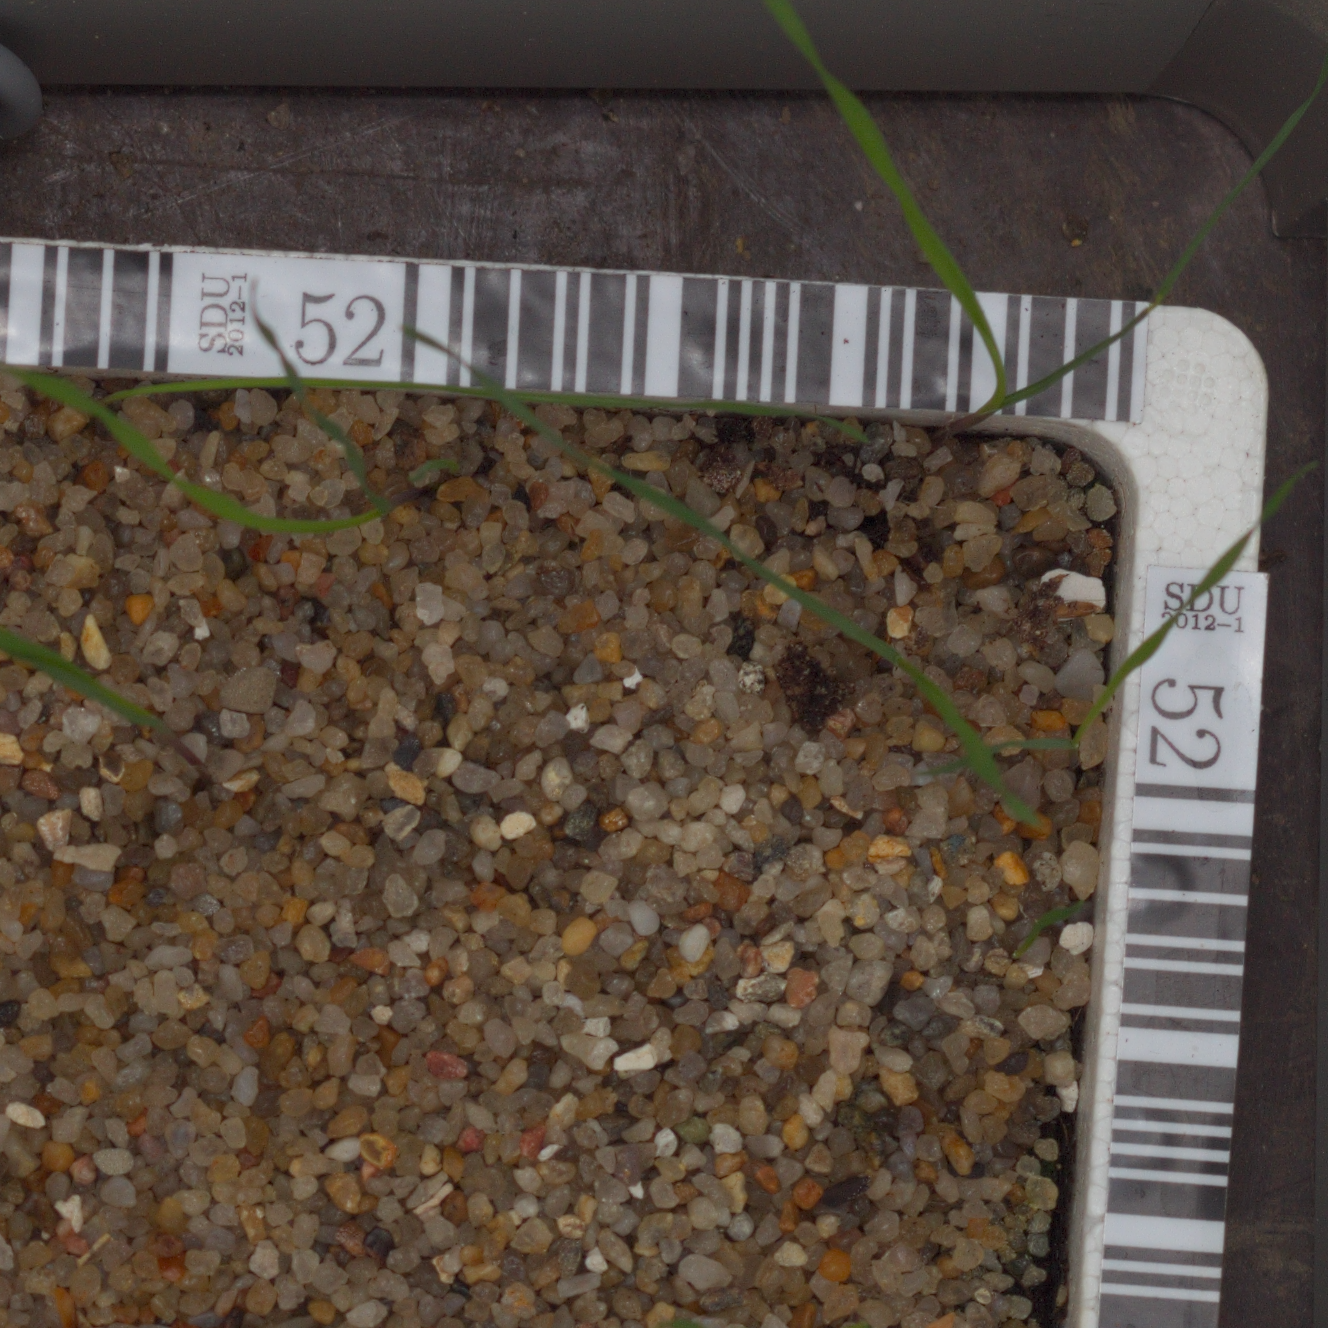
\includegraphics[width=6cm, height=6cm]{black_grass_1} 
		\label{fig_res_diff_a}}
	}
    \qquad
    \subfigure[\textit{Loose Silky-bent}]{
		{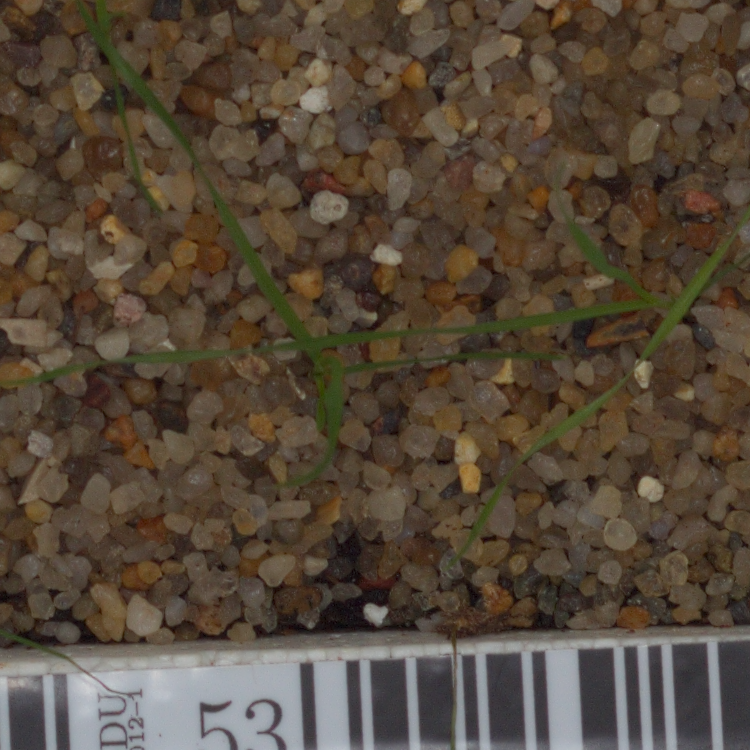
\includegraphics[width=6cm, height=6cm]{loose_silky_bent_1} 
		\label{fig_res_diff_b}}
	}
    \caption{Схожесть образцов классов}%
    \label{fig_res_diff}
\end{figure}

\indent{Предполагается, что качество классификации можно существенно улучшить, изменив метод сегментации. На данный момент не удается выделить части стебля растения, близкие к земле. Задать порог цвета для основания растения затруднительно, поэтому более тонкие отличия между растениями, как на примере \ref{fig_res_diff} (\ref{fig_res_diff_a} обладает не зеленым основанием), могут затеряться.}

\indent{Также можно рассмотреть другие группы признаков, к примеру, текстурные, но возникает проблема с изображениями очень низкого разрешения, где отличительной текстуры не наблюдается. Поэтому необходимо найти подход, учитывающий несовершенства исходных данных.}

\newpage
\begin{thebibliography}{}
	\bibitem{bib_1} Giselsson, T., Jørgensen, R., Jensen, P., Dyrmann, M., and Midtiby, H. (2017). A Public Image Database for Benchmark of Plant Seedling Classification Algorithms. 
	\bibitem{bib_2} Bradski, G. (2000). The OpenCV Library. Dr. Dobb's Journal of Software Tools.
	\bibitem{bib_3} Oliphant, T. E. (2006). A guide to NumPy (Vol. 1). Trelgol Publishing USA.
	\bibitem{bib_4} Panja, D., Poppe, R. (2018). INFOIBV. Image Processing course, Universiteit Utrecht.
	\bibitem{bib_5} Wojnar, L., Kurzydłowski, K. J. et al. (2000). Practical Guide to Image Analysis, ASM International.
	\bibitem{bib_6} Suzuki, S. and Abe, K. (1985). Topological Structural Analysis of Digitized Binary Images by Border Following.
	\bibitem{bib_7} Pedregosa et al. (2011). Scikit-learn: Machine Learning in Python
	\bibitem{bib_8} Chih-Wei Hsu, Chih-Chung Chang, Chih-Jen Lin (2003). A Practical Guide to Support Vector Classification.
\end{thebibliography}

\end{document}{}